% !TEX root = main.tex

\section{图像分割}
图像分割一般基于亮度值的两种基本特性(\textbf{不连续性}和\textbf{相似性})来分割。

\begin{definition}[分割]
令$R$为全图,可将分割看作$R$划分为$n$个子区域$R_1,R_2,\ldots,R_n$的过程:
\begin{enumerate}
	\item $\disp\bigcup_{i=1}^n R_i=R$
	\item $R_i$是一个连通区域
	\item $R_i\cap R_j=\varnothing$
	\item $Q(R_i)=TRUE$
	\item $Q(R_i\cup R_j)=FALSE$,对于任何$R_i$和$R_j$的邻接区域
\end{enumerate}
其中,$Q(R_k)$为定义在集合$R_k$的点上的逻辑属性
\end{definition}

\subsection{点检测与线检测}
点检测(Laplace算子)
\begin{center}
\begin{tabular}{|c|c|c|}\hline
1 & 1 & 1\\\hline
1 & -8 & 1\\\hline
1 & 1 & 1
\end{tabular}
\end{center}
若作用算子后的图像$|R(x,y)|\geq T$,则记为$1$。

线检测
\begin{figure}[H]
\centering
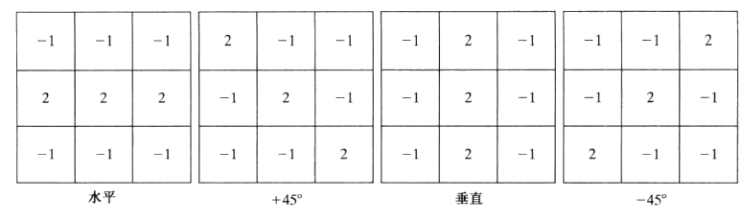
\includegraphics[width=0.9\linewidth]{fig/line_detect.png}
\end{figure}

\subsection{边缘检测}
傅里叶变换无法刻画边缘,只知道高频成分,不知道高频在哪里。
一种方法是局部傅里叶变换,衍生出小波变换(就是要构造一种高通滤波器):有震荡信号的位置(小范围震荡且积分为0),可以刻画边缘。

台阶、斜坡、屋顶边缘模型如下。
\begin{figure}[H]
\centering
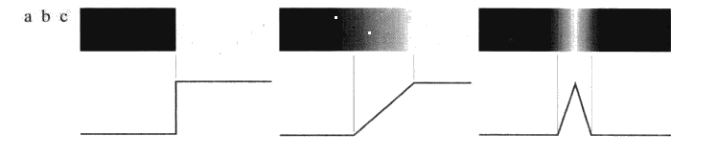
\includegraphics[width=0.9\linewidth]{fig/edge_model.png}
\end{figure}

边界是封闭的边缘。

二阶导数会增大噪声,因此做边缘检测之前应该先抑制噪声(平滑)。
\begin{figure}[H]
\centering
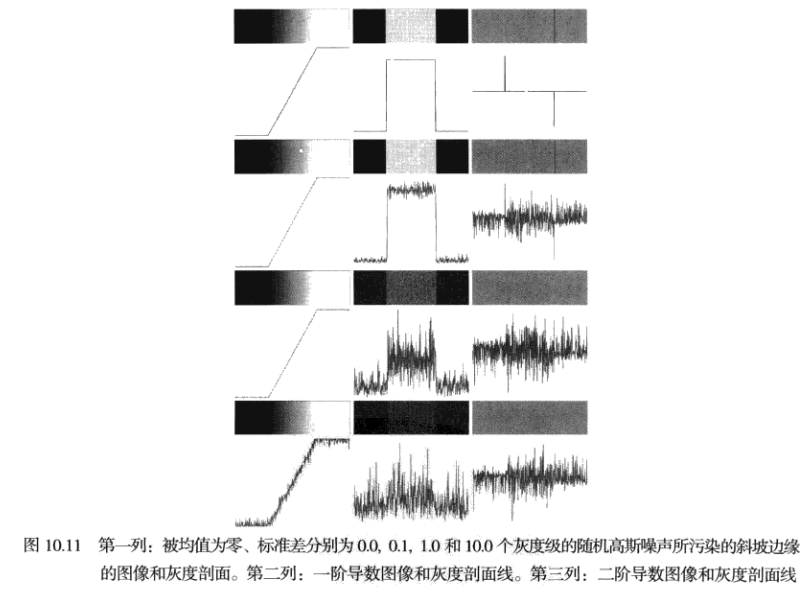
\includegraphics[width=0.9\linewidth]{fig/edge_detect_noise.png}
\end{figure}

边缘检测算子
\begin{figure}[H]
\centering
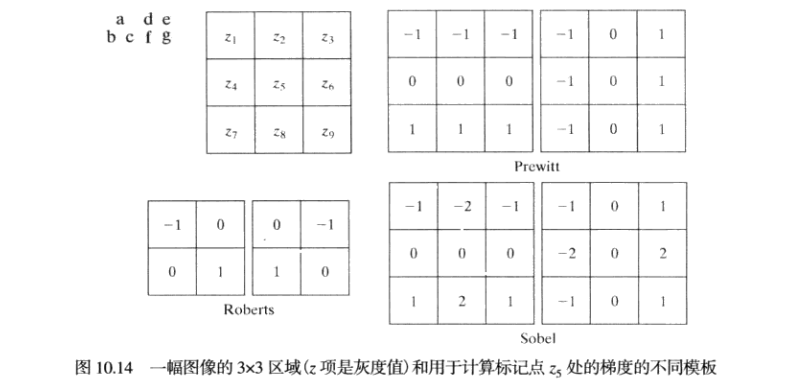
\includegraphics[width=0.9\linewidth]{fig/edge_detect_op.png}
\end{figure}

Marr-Hildreth边缘检测器
\[\nabla^2 G(x,y)=\lrs{\frac{x^2+y^2-2\sigma^2}{\sigma^4}}\ee^{-\frac{x^2+y^2}{2\sigma^2}}\]
即高斯拉普拉斯(LoG)变换。

(高斯函数的微分就是一种小波,做微分后负号与负号抵消)